In questo esperimento si vuole studiare un amplificare in classe AB. Il circuito, riportato in Figura \ref{fig:CircuitFac4}, è alimentato dalla tensione duale $\pm V_{CC}=\pm 12V$.
\begin{figure}[H]
    \centering
    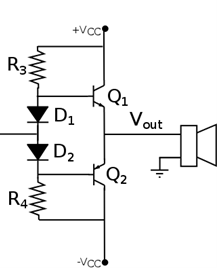
\includegraphics[width=0.3\linewidth]{images/CircuitFac4.png}
    \caption{Schema circuito}
    \label{fig:CircuitFac4}
\end{figure}
I due diodi PN (polarizzati dalle resistenze $R_3$ e $R_4$) creano una differenza di potenziale circa uguale a $0.6 V$ tra il segnale di ingresso e la base dei transistor $Q_1$ e $Q_2$. Di conseguenza, basta che il segnale di ingresso superi di poco la tensione nulla perché uno dei due transistor di uscita entri in conduzione. Rispetto allo stadio in classe B, questo schema presenta una distorsione di crossover trascurabile.
\subsubsection{Dimensionamento circuito}
Si è scelto i valori di $R_3$ e $R_4$ in modo tale da da garantire una corrente di $1 mA$ sui diodi $D_1$ e $D_2$ (con tensione di ingresso nulla).\\
Si è scelto quindi
\begin{equation*}
    R_3=R_4=10k\Omega
\end{equation*}
\subsection{Procedura di valutazione e risultati}
Mantenendo la tensione in ingresso $V_{in}=0$, con il multimetro sono state misurate le correnti sulle resistenze $R_3$ e $R_4$
\begin{equation*}
    I_{R_3}=1.14mA\quad I_{R_4}=1.21mA
\end{equation*}
e la caduta di tensione sui due diodi $D_1$ e $D_2$
\begin{equation*}
    V_{D_1}=0.612V\quad V_{D_2}=0.606V
\end{equation*}
\clearpage 
Il generatore di forma d'onda è stato impostato con il seguente segnale:
\begin{itemize}
    \item Forma d'onda: sinusoidale
    \item Ampiezza iniziale: $1V$ picco-picco
    \item Frequenza: $220Hz$ (nota La)
\end{itemize}
Abbiamo impostato l'oscilloscopio per misurare il segnale di ingresso e di uscita. Riportiamo in Figura \ref{fig:scope_15} la schermata dell'oscilloscopio con i due segnali
\begin{figure}[H]
    \centering
    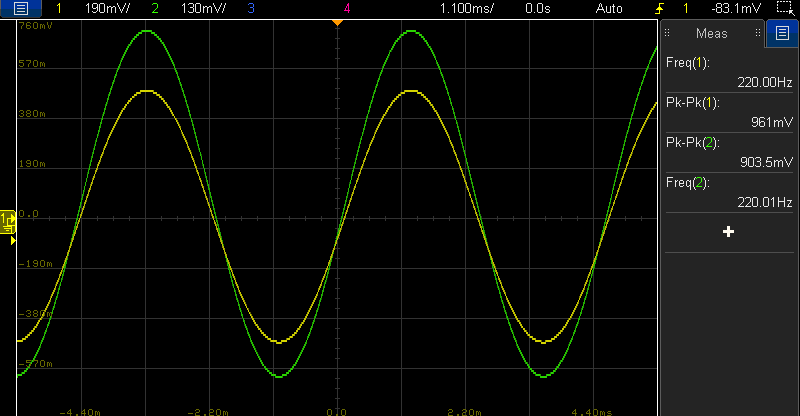
\includegraphics[width=0.7\linewidth]{images/scope_15.png}
    \caption{Segnale in ingresso e in uscita dal circuito}
    \label{fig:scope_15}
\end{figure}
Attraverso i cursori dell'oscilloscopio è stata misurata la distorsione di crossover. Come si vede dal dettaglio della Figura \ref{fig:scope_16} è risultato che non è presente alcuna distorsione. Infatti entrambi i diodi a riposo sono polarizzati in zona diretta e permettono di avere i BJT in zona attiva.
\begin{figure}[H]
    \centering
    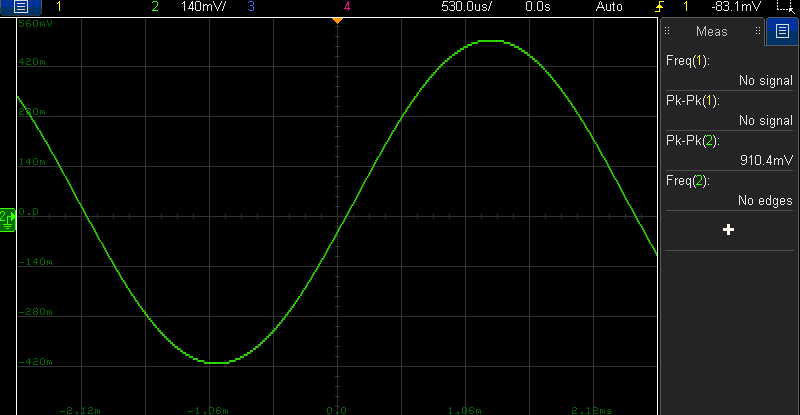
\includegraphics[width=0.7\linewidth]{images/scope_16.png}
    \caption{Dettaglio segnale di uscita}
    \label{fig:scope_16}
\end{figure}

\section{Conclusioni}
Commentare brevemente i risultati ottenuti nei tre esperimenti; confrontare i tre stadi amplificatori in termini di prestazioni e efficienza (a livello teorico)